% 第 17 题圆台图：按固定源 PDF 矢量路径换算（1 pt → 0.03515 cm）。
% 原点取图组左下（源页 (962.09, 656.43) pt），y 向上。轴竖直（上下底椭圆圆心同 x=85.40）。
% 上底整椭圆实线（r 42.70/8.22）；下底：前半（近侧）下半弧实线、后半（远侧）上半弧虚线（r 85.40/16.45）；
% 左母线＝左侧轮廓，右母线 FB。虚线 7 条：AC（过 O 的直径）、OB、AB、BC、CE、CF、GH（G、H 为 EC、FB 中点）。
% 两圆心各画实心圆点；字母位置按源字形外接框中心定位（显式坐标）。
% 注：源图未按题设 AB=BC 精确作图（矢量实测 |AB|:|BC|≈1.45:1），照源描摹，不得据图反推题设。
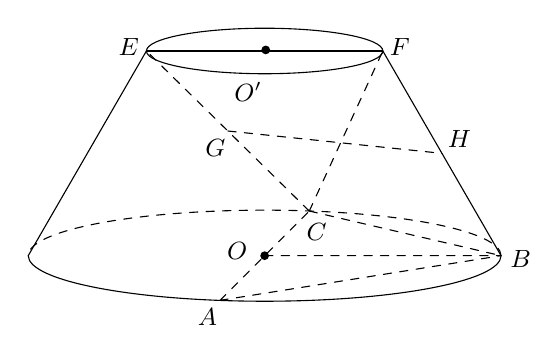
\begin{tikzpicture}[line cap=round,line join=round,font=\small,x=0.03515cm,y=0.03515cm]
% ===== 虚线先画 =====
\draw[dash pattern=on 2.99pt off 2.99pt]
  (69.26,10.70)--(101.53,42.97)   % AC（直径，过 O）
  (85.40,26.84)--(170.80,26.84)   % OB
  (69.26,10.70)--(170.80,26.84)   % AB
  (101.53,42.97)--(170.80,26.84)  % BC
  (101.53,42.97)--(42.70,100.79)  % CE（母线）
  (101.53,42.97)--(128.10,100.79) % CF（母线）
  (72.12,71.88)--(149.45,63.81);  % GH（EC、FB 中点连线）
% 下底后半（远侧）上半弧
\draw[dash pattern=on 2.99pt off 2.99pt] (170.80,26.84) arc[start angle=0,end angle=180,x radius=85.40,y radius=16.45];
% ===== 实线 =====
% 上底整椭圆
\draw (85.40,100.79) ellipse (42.70 and 8.22);
% 上底直径 EF
\draw (42.70,100.79)--(128.10,100.79);
% 两条母线（左轮廓、右母线 FB）
\draw (0,26.84)--(42.70,100.79);
\draw (128.10,100.79)--(170.80,26.84);
% 下底前半（近侧）下半弧
\draw (0,26.84) arc[start angle=180,end angle=360,x radius=85.40,y radius=16.45];
% ===== 圆心圆点 =====
\fill (85.80,101.17) circle (1.58);
\fill (85.40,26.84) circle (1.58);
% ===== 标注（显式坐标，照源字形框中心）=====
\node[anchor=center,inner sep=0] at (36.34,102.39) {$E$};
\node[anchor=center,inner sep=0] at (134.23,102.39) {$F$};
% O′ 下移至椭圆下弧之下（源位与弧相切，400 dpi 连通域实证并入；照清晰度优先原则微调）
\node[anchor=center,inner sep=0] at (79.5,86.0) {$O'$};
\node[anchor=center,inner sep=0] at (67.58,65.87) {$G$};
\node[anchor=center,inner sep=0] at (155.78,69.07) {$H$};
\node[anchor=center,inner sep=0] at (64.72,4.66) {$A$};
\node[anchor=center,inner sep=0] at (104.23,35.44) {$C$};
\node[anchor=center,inner sep=0] at (177.94,25.74) {$B$};
% O 左下移（源位紧贴圆心点与 AC 线，同上微调）
\node[anchor=center,inner sep=0] at (75.5,28.5) {$O$};
\end{tikzpicture}
